\chapter{Le sujet du stage}
\section{Géochronologie} %"Un peu de Géochronologie..." ?
%TODO : Parler du mass spectrometer!
Le carbone 14 est un isotope populairement connu comme permettant de dater un objet. Il n'est cependant pas le seul. L'uranium et le plomb permettent aussi, dans des conditions particulières, de dater une couche du globe terrestre.

Quand un volcan entre en éruption, en plus de la lave expulsé de son cratère, celui-ci crache aussi des \textit{zircons}. Un zircon est un cristal qui, lorsqu'il est créé, ne comporte que de l'uranium. Il est important de noter que ces cristaux sont des capsules hermétiques : rien n'en sortira et n'y rentrera. Ces zircons atterrissent dans la lave et se retrouve emprisonnés. 

Le temps passe, de nouvelles couches se forment, au dessus de la lave. L'uranium à l'intérieur des zircons se décompose en plomb, à une vitesse bien définie et connue des chercheurs. 

Des millions d'années plus tard, quand les chercheurs se posent la question de l'âge d'une couche terrestre au pied d'un volcan, ils cassent sur place des énormes blocs de lave solidifée. Grâce à un procédé complexe, ils en extraient ensuite les zircons. Dans ces zircon se trouve une partie de l'uranium intacte et une partie de l'uranium transformé en plomb. En mesurant le rapport entre l'uranium et le plomb présent dans les zircons, les chercheurs peuvent déterminer l'âge de la couche terrestre où ils ont été trouvés.

Le but du laboratoire \textit{CIRDLES} est d'aider les chercheurs dans cette tâche précise et complexe.

\section{Le projet : Topsoil}
Le logiciel sur lequel j'ai travaillé s'appelle \textit{Topsoil}. Il permet de produire ce genre de graphiques :
\begin{center}
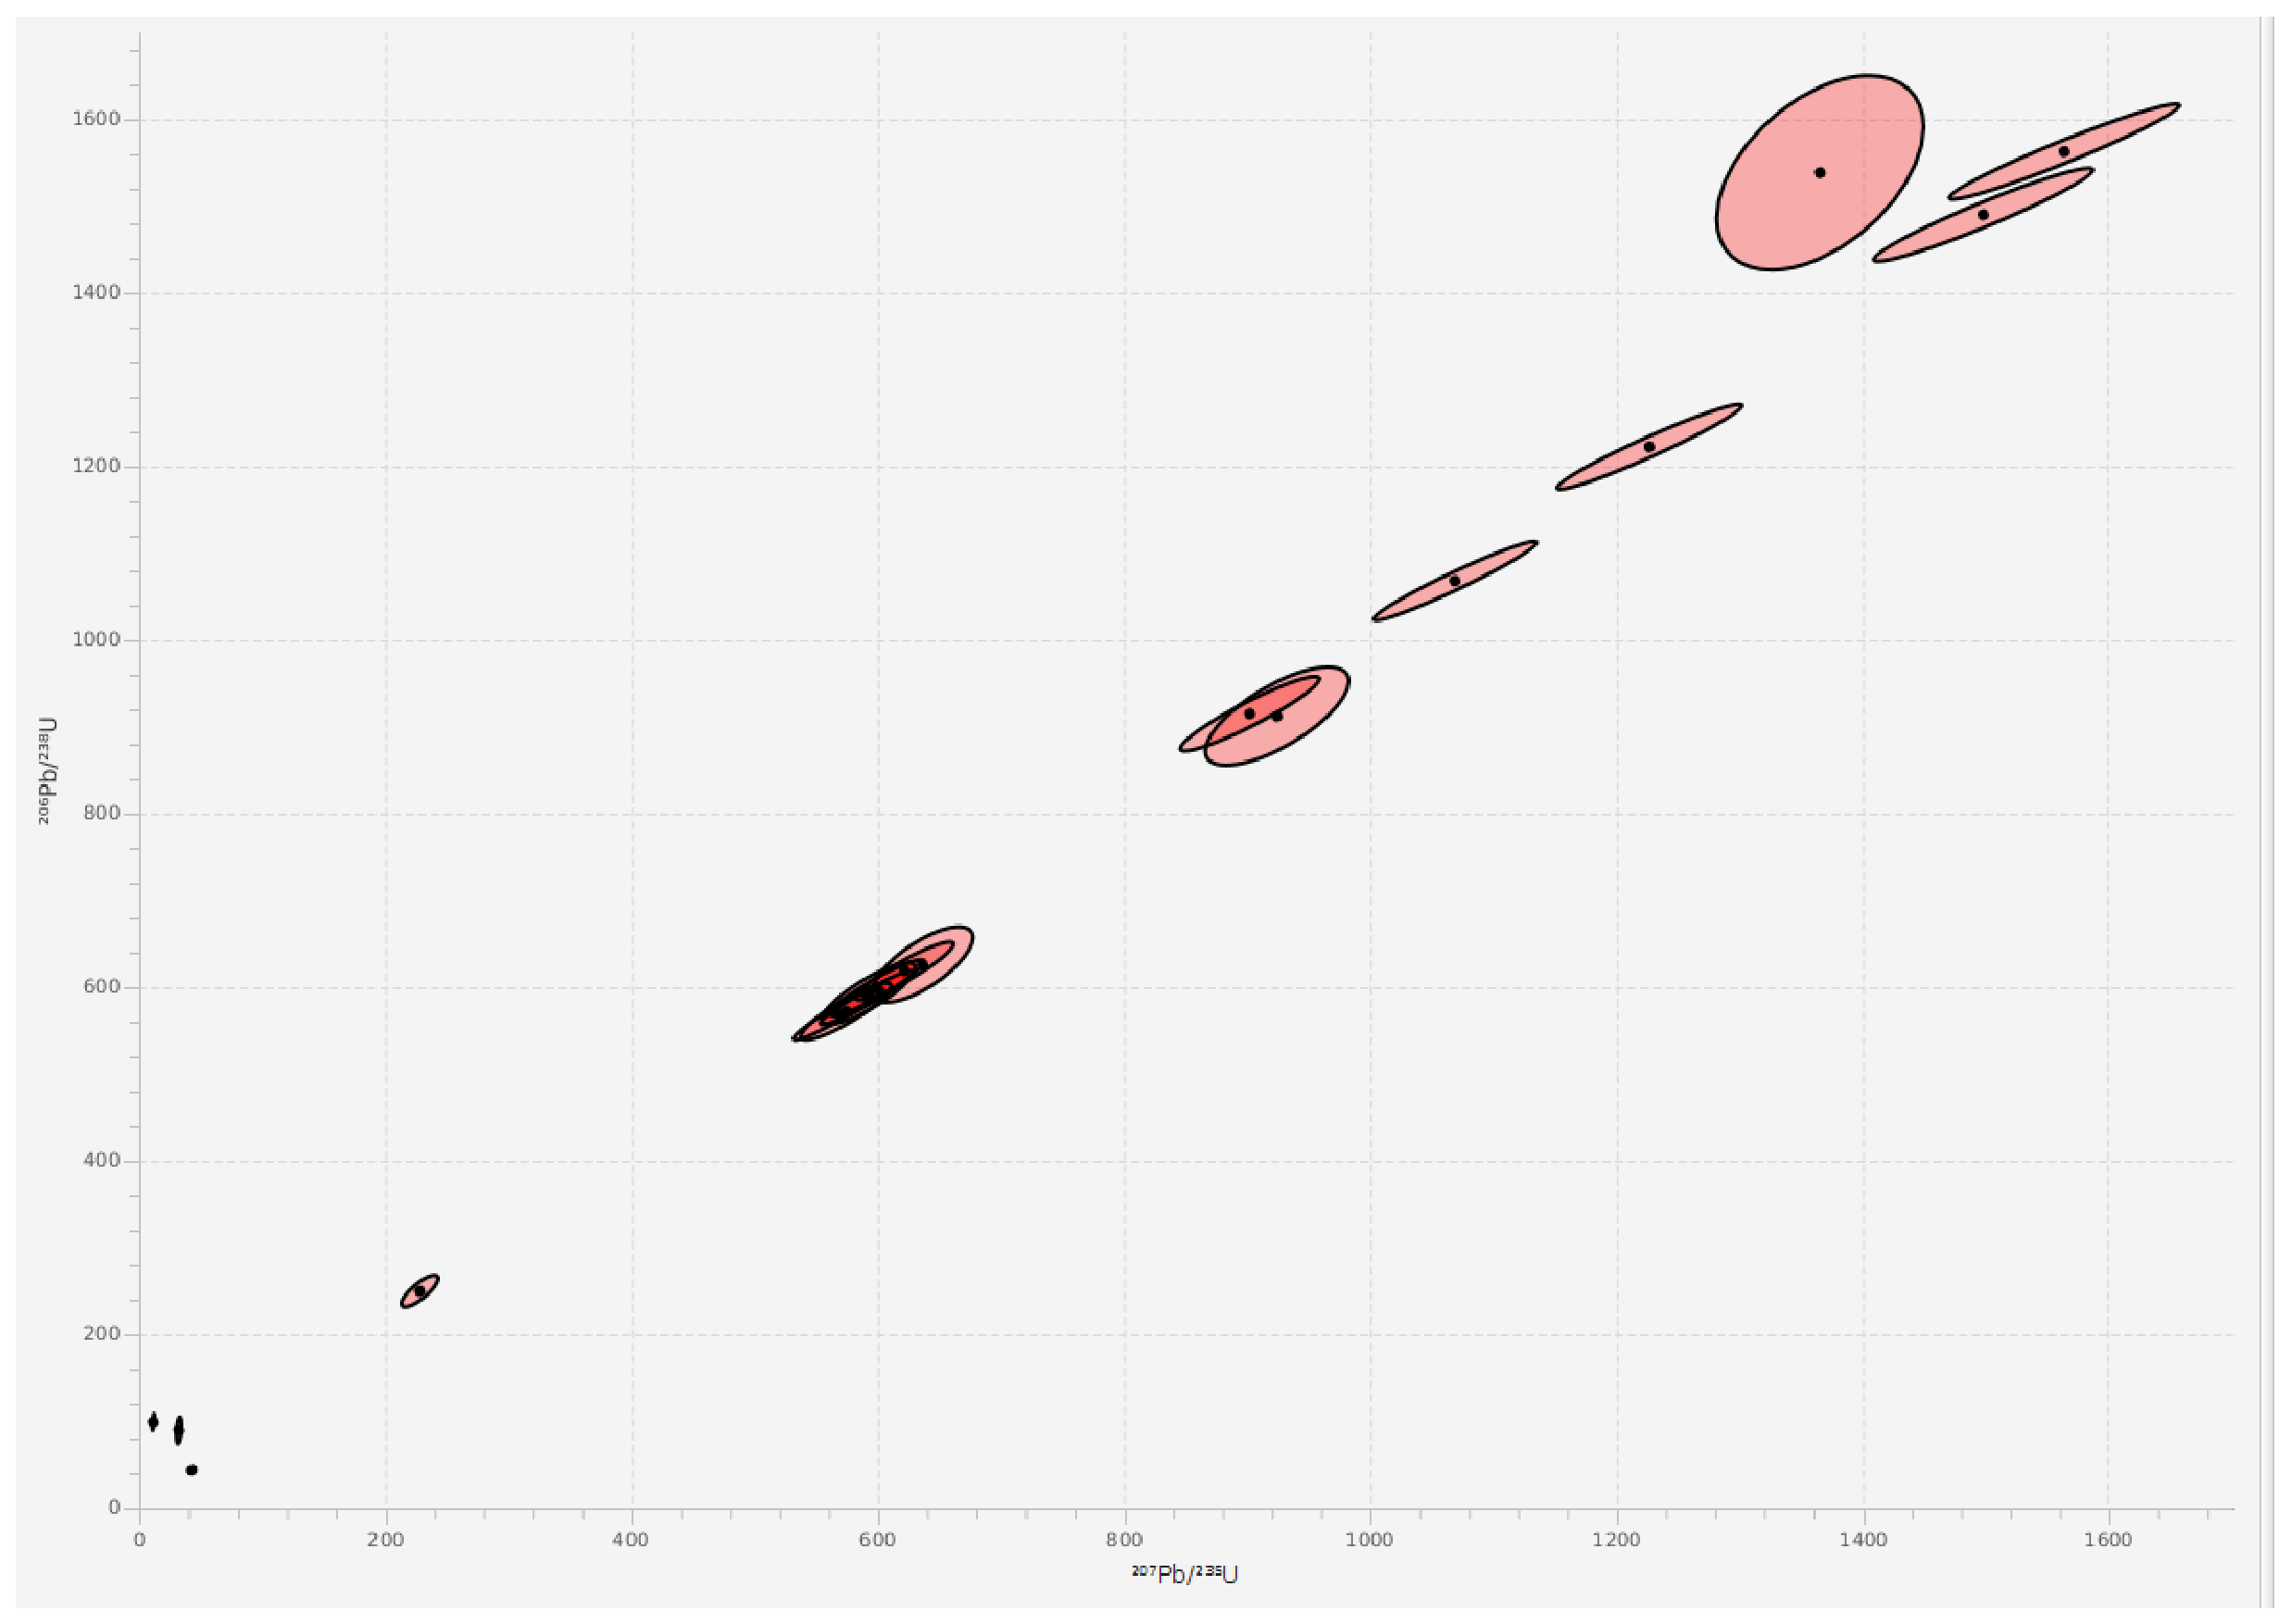
\includegraphics[width=15cm]{./illustrations/graphique.eps}
\end{center}
Il remplace un autre logiciel nommé \textit{Isotop}.

\subsection{Les ellipses d'erreurs}
%parler de la façon dont on insère les données dans le tableau

\begin{quote}
Un isotope est, pour faire simple, une déclinaison d'un élément chimique. Tous les éléments chimiques, comme l'uranium et le plomb, ont plusieurs isotopes.
\end{quote}

En réalité, les chercheurs ne comparent pas \emph{le} ratio entre l'uranium et le plomb dans un zircon. Ils comparent \emph{les} ratios entre \emph{différants isotopes} d'uranium et de plomb présent dans le zircon.
Une ellipse représentée sur ce schéma montre la relation entre deux de ces ratios.

Si l'on arrivait à mesurer précisemment ces ratios, ces ellipses ne seraient que des points. Les deux ratios donneraient l'abscisse et l'ordonnée de ces points. Mais, en physique, la précision absolue n'existe pas. Par exemple, prenez une règle et mesurez le côté d'une table dix fois au millimètre près. Vous n'obtiendrez jamais la même mesure. Vous pouvez par contre statistiquement déterminer une fourchette dans laquelle se trouve la vraie longueur de la table, entre 10.5 cm et 10.7cm par exemple. Le même principe s'applique avec les ratios : les géochronologistes ne trouvent pas une valeur précise pour chaque ratio mais une fourchette dans laquelle cette valeure est. Ces deux fourchettes et la corrélation des deux ratios donne l'ellipse. Les chercheurs se servent donc de ce schéma pour étudier l'inexactitude des mesures du spectromètre de masse.

Puisque les scientifiques font ces mesures sur plusieurs zircons pour une seule couche terrestre, ils entrent toutes ces mesures sur le même schéma, d'où la présence de multiples ellipses.

La ligne qui traverse le schéma est une ligne de temps, appelée ligne de Concordia. C'est par rapport à elle que les chercheurs déterminent l'âge des différents ratios présents sur le schéma. Il en existe plusieurs types.

\subsection{Remplacer \textit{Isoplot}}
Après trente années de bon et loyaux services à la communauté scientifique, Ken Ludwig a décidé de d'arrêter le développement d'\textit{Isoplot}, le plug-in permettant à Excel de tracer entre autre le schema expliqué dans la section précédante.

Ce plug-in était devenu encombrant pour les géochronologistes depuis quelques années pour les raisons suivantes :

\begin{itemize}
\item Il ne fonctionne correctement que sur les versions 97 et 2003 de la suite Office. Une déclinaison du plug-in a été réalisée pour des versions plus récentes mais elle est plus lente et supporte moins de fonctions. Cela force les laboratoire ayant besoin de ses services à rester sur de vieux PC et de vieux systèmes d'exploitation comme Windows XP qui ne sont plus supportés par Microsoft et donc dangereux à utiliser.
\item Il ne génère des schémas que dans une feuille Excel et ne supporte pas l'export vers des logiciels de traitement vectoriel. Les géochronologistes ont besoin de cette fonctionnalité pour intégrer les schémas dans leur papier ou leurs présentations.
\item Esthétiquement parlant, les schémas produits ne sont pas très réussis
\item Un plug-in Excel, écrit en \textit{Visual Basic}, un vieux langage de programation qui n'est plus très utilisé est voué à vieillir sans être mis à jour. Ce code est à usage uniquem, il n'est pas possible de l'intégrer dans une autre solution. De plus, le code n'est pas libre, ce qui rend la continuation du travail impossible.
\end{itemize}

La communauté était donc avide d'un remplacement pour ce vieux logiciel et le docteur Bowring voulait la lui la fournir. Encore fallait qu'il trouve des clients directement intéressés. Ce n'est qu'en se faisant endosser par des collègues chercheurs que son laboratoire pourrait avoir des fonds de la \textit{National Science Fundation}.

C'est alors qu'un géochronologiste australien, Keith Sircombe, lui à envoyé un cas d'utilisation précis à réaliser. Le docteur Bowring nous a mis, John Zeringue et moi, immédiatement au travail sur l'implémentation de ce cas d'utilisation. Si l'on arrivait à convaincre Sircombe que nous pouvions faire un travail correct, nous aurions les fonds.

\subsection{Au delà d'\textit{Isoplot}, la création d'un outil durable}
Les projets du Docteur Bowring ne s'arrêtent cependant pas au simple remplacement d'\textit{Isoplot}. Son ambition est de créer un outil de tracé durable pour un grand nombre de schémas, et utilisable dans un grand nombre de cas.

Afin de le rendre durable, plusieurs choix ont été faits : 
\begin{itemize}
\item Un langage majeur et stable, Java, a été choisi pour le développement du logiciel.
\item Ce projet est pensé non seulement dans l'optique de faire un logiciel, mais aussi de créer une librairie de tracé, réutilisable dans n'importe quel projet, notamment \textit{U\_Pb\_Redux}, le logiciel programmé par le Docteur Bowring.
\item Le projet sera libre et conduit par les demandes et les besoins de la communauté de géochronologistes
\end{itemize}
